\documentclass{article}
\usepackage{tikz}
\usepackage{circuitikz}

\begin{document}

\begin{center}
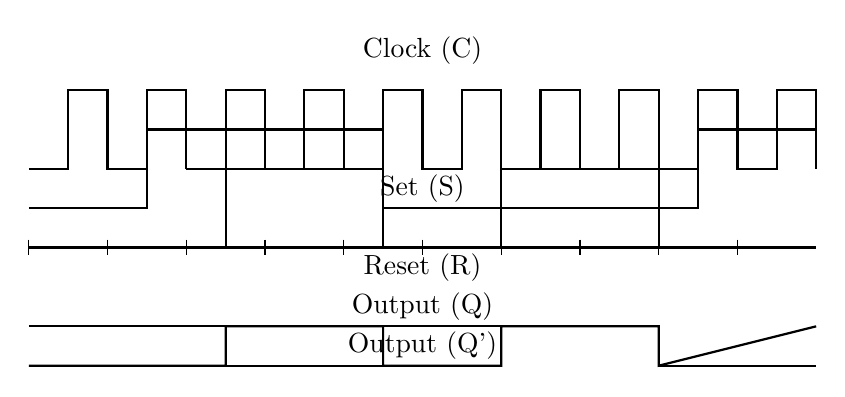
\begin{tikzpicture}
% Time axis
\draw[thick] (0,0) -- (10,0);
\foreach \x in {0,1,2,3,4,5,6,7,8,9} {
    \draw (\x,0.1) -- (\x,-0.1);
}

% Clock signal (C)
\draw[thick] (0,1) -- (0.5,1) -- (0.5,2) -- (1,2) -- (1,1) -- (1.5,1) -- (1.5,2) -- (2,2) -- (2,1);
\draw[thick] (2,1) -- (2.5,1) -- (2.5,2) -- (3,2) -- (3,1) -- (3.5,1) -- (3.5,2) -- (4,2) -- (4,1);
\draw[thick] (4,1) -- (4.5,1) -- (4.5,2) -- (5,2) -- (5,1) -- (5.5,1) -- (5.5,2) -- (6,2) -- (6,1);
\draw[thick] (6,1) -- (6.5,1) -- (6.5,2) -- (7,2) -- (7,1) -- (7.5,1) -- (7.5,2) -- (8,2) -- (8,1);
\draw[thick] (8,1) -- (8.5,1) -- (8.5,2) -- (9,2) -- (9,1) -- (9.5,1) -- (9.5,2) -- (10,2) -- (10,1);
\node at (5,2.5) {Clock (C)};

% Set input (S)
\draw[thick] (0,0.5) -- (1.5,0.5) -- (1.5,1.5) -- (4.5,1.5) -- (4.5,0.5) -- (8.5,0.5) -- (8.5,1.5) -- (10,1.5);
\node at (5,0.75) {Set (S)};

% Reset input (R)
\draw[thick] (0,0) -- (2.5,0) -- (2.5,1) -- (4.5,1) -- (4.5,0) -- (6,0) -- (6,1) -- (8,1) -- (8,0) -- (10,0);
\node at (5,-0.25) {Reset (R)};

% Outputs Q and Q'
\draw[thick] (0,-1) -- (2.5,-1) -- (2.5,-1.5) -- (4.5,-1.5) -- (4.5,-1) -- (8,-1) -- (8,-1.5) -- (10,-1.5);
\node at (5,-0.75) {Output (Q)};

\draw[thick] (0,-1.5) -- (2.5,-1.5) -- (2.5,-1) -- (4.5,-1) -- (4.5,-1.5) -- (6,-1.5) -- (6,-1) -- (8,-1) -- (8,-1.5) -- (10,-1);
\node at (5,-1.25) {Output (Q')};

\end{tikzpicture}
\end{center}

\end{document}
